\section{Sensorer}\label{sensorer}
Dette afsnit beskriver de sensorer der kan være interessante at bruge som datakilder. 

\paragraph{Kamera}
Kameraet kan tage billeder og billedesekvenser i form af video optagelse.
På smartphones er der typisk to kameraer af forskellig kvalitet; et højere kvalitets kamera på bagsiden, samt et lavere kvalitets kamera på forsiden (samme side som skærmen).

\paragraph{Accelerometer}
Accelerometeret måler accelerationen i x, y og z akserne i et koordinatsystem, som vist på \cref{analyse:accelerometer:koo}.
Accelerometret kan konceptuelt forstås som en kugle der ruller rundt i et rum hvor væggene kan måle den g-kraft de bliver påvirket med.
På \cref{analyse:accelerometer:kraft} ses dette konceptuelle rum med påvirkning fra tyngdekraften. 
Sensoren vil i dette tilfælde rapportere en g-kraft i z-aksens retning.

\begin{figure}[h]
	\centering
	\begin{subfigure}[b]{0.47\textwidth}
		\centering
		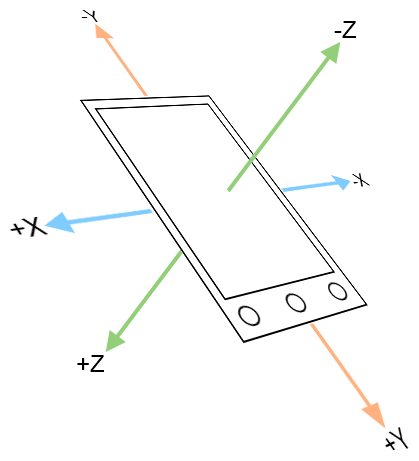
\includegraphics[width=.6\textwidth]{accelerometer-telefon}
		\caption{Koordinatsystem i forhold til smartphonen}
		\label{analyse:accelerometer:koo}
	\end{subfigure}
	~
	\begin{subfigure}[b]{0.47\textwidth}
		\centering
		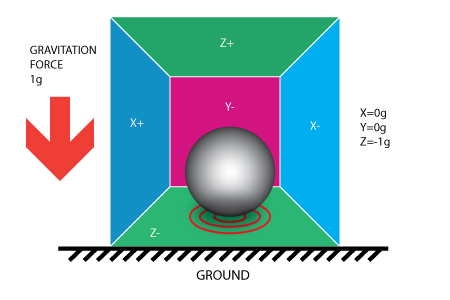
\includegraphics[width=\textwidth]{accelerometer}
		\caption{Konceptuel tegning af et accelerometers virkemåde. Illustration fra \citep{accelerometer}}
		\label{analyse:accelerometer:kraft}
	\end{subfigure}
	\caption{}
	\label{accelerometer}
\end{figure} 

\paragraph{GPS}
Gennem GPS gives en lokation bestående af breddegrad og længdegrad, samt en pejling.
Ved at differentiere positionen ift. tid kan man beregne hastigheden og ved at differentiere igen kan man beregne accelerationen.
Denne sensor er dog ofte utilgængelig når enheden er indendørs, da de signaler der bruges til GPS positionsbestemmelse ikke kommer ind i de fleste bygninger.

\paragraph{Mikrofon}
Mikrofonen kan optage omgivelserne ved at konvertere akustisk lyd til elektriske signaler.
Kvaliteten og følsomheden af denne kommer an på selve smartphonen, idet mikrofonenerne er forskellige afhængigt af typen af smartphone. 

\paragraph{Lys-sensor}
Lys-sensoren kan måle belysningsstyrken, altså intensiteten af lyset, på en flade.
Enheden for dette er lux.

\paragraph{Pulsmåler}
Pulsmåleren måler pulsen i hjerteslag per minut.
Dette gøres ved enten at sende en elektrisk puls igennem et ledende materiale mod huden eller med en optisk sensor der også holdes mod huden.
Den mest præcise måling fås hvis sensoren sidder spændt omkring brystet, mens sensorer der måler enten på håndleddet eller fingeren er mindre præcise \citep{burke1998precision}.

\paragraph{Galvanisk hud respons}
Galvanisk hud respons (GHR) sensoren siger noget om hvor god huden er til at lede strøm, da huden er mere strøm-ledende jo mere der svedes.
